\documentclass{article}

\usepackage{graphicx}
\usepackage[labelformat=empty]{caption}
\usepackage{tocloft}
\usepackage[hidelinks,
            colorlinks=true,
            linkcolor=blue,
            urlcolor=blue,
            bookmarks=true,
            bookmarksopen=true]{hyperref}

\setlength{\parindent}{0pt}

\title{Assembly Guide}
\author{D-Lab Team Mexico}

\begin{document}

\maketitle

\pagenumbering{arabic}
\tableofcontents
\vspace{2cm} 
\clearpage
\pagenumbering{arabic}
\section{Software}\label{sec:software}
\subsection{Installing the Arduino IDE}
To install the Arduino IDE, visit the official Arduino website at the following link:

\href{https://www.arduino.cc/en/software}{https://www.arduino.cc/en/software}

\noindent
Download the version appropriate for your operating system and follow the installation instructions provided on the website.

\subsection{Installing the libraries}


Once you have opened the Arduino IDE, click on the ``Library Manager'' in the left bar. It has the following icon:

\vspace{1em}
\begin{center}
    
\includegraphics[width=0.2\textwidth]{../images/library_manager.png}
\end{center}

Now look for the following libraries:

\begin{itemize}
    \item Adafruit GFX Library, by Adafruit: say yes to installing all dependencies (which will be only Adafruit BusIO).
    \item MCUFRIEND\_kbv, by David Prentice.
    \item SD, by Arduino and SparkFun.
\end{itemize}

\noindent
Now, navigate to the location of your computer where the Arduino IDE keeps the ``Arduino Sketchbook'' folder. If you're unsure about where it is, there are some common paths:

\begin{itemize}
    \item Windows: C:\textbackslash Users\textbackslash [your username]\textbackslash Documents\textbackslash Arduino
    \item Mac: \(\sim \)/Documents/Arduino
    \item Linux: \(\sim \)/Arduino
\end{itemize}

Inside that folder, look for the folder ``libraries''. Click on ``MCUFRIEND\_kbv'' and then on ``utils''. Now, do the following:

\begin{itemize}
    \item Edit \texttt{mcufriend\_shield.h}: in the first line, remove the two slashes (\texttt{//}) before \texttt{\#define USE\_SPECIAL}.
    \begin{figure}[h]
        \centering
        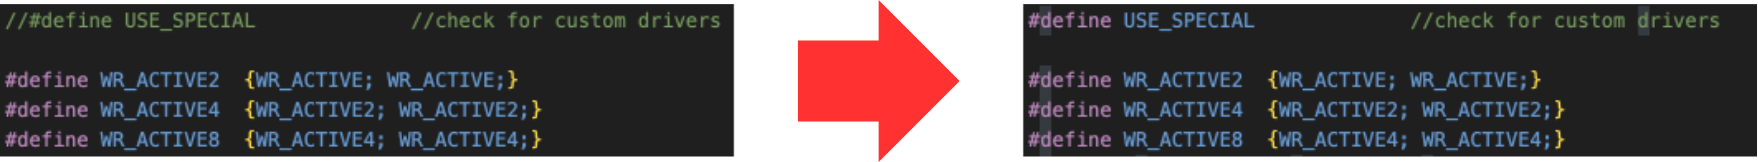
\includegraphics[width=1.3\textwidth]{../images/mcufriend_shield.png}
        \end{figure}
    \item Edit \texttt{mcufriend\_special.h}: in the 6th line, remove the two slashes (\texttt{//}) before \texttt{\#define USE\_MEGA\_16BIT\_SHIELD}.
\end{itemize}

\newpage
\subsection{Downloading the code}
To download the code, go to the following link:

\href{https://github.com/CarolinaMoura/assistive-voices}{https://github.com/CarolinaMoura/assistive-voices}

Once in the page, click on the green button that reads ``Code'', and then on ``Download ZIP'':

\begin{figure}[h]
\centering

\includegraphics[width=0.3\textwidth]{../images/code.png}
\caption{The ``code'' button.}
\end{figure}

\begin{figure}[h]
\centering
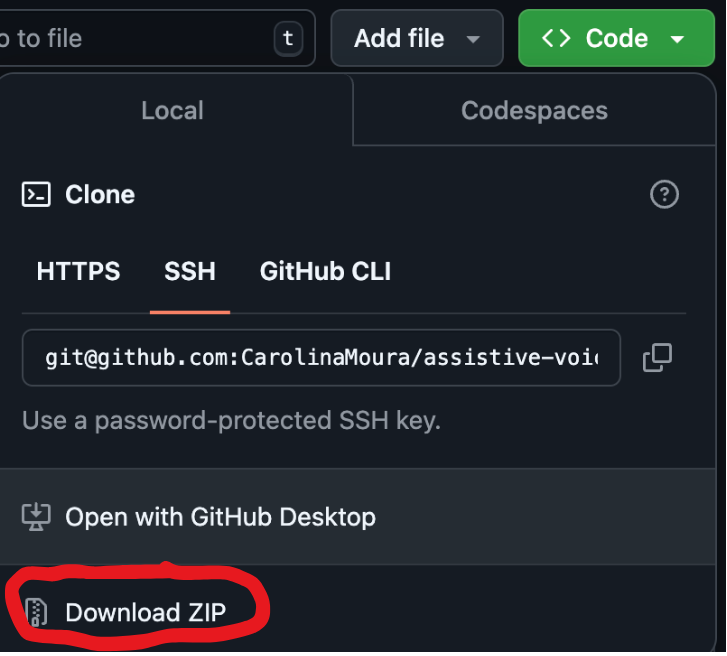
\includegraphics[width=0.5\textwidth]{../images/download_zip.png}
\caption{The ``Download ZIP'' option.}
\end{figure}

Now, unzip the downloaded folder. Inside the unzipped folder, you will find a folder named ``main''. This folder contains the code for the project.

\begin{itemize}
    \item Go inside the ``main'' folder.
    \item Double-click the file named ``main.ino''. This should open the Arduino IDE with the code.
    \item If the file does not open automatically, right-click on ``main.ino'' and select ``Open with...''. Choose the Arduino IDE from the list of available programs.
\end{itemize}

Now you have the code open in the Arduino IDE.

\newpage
\section{SD cards}\label{sec:sdcards}
Now we need to load the SD cards with the necessary files. You must have 2 SD cards, one for the images and another for the audio files. It doesn't matter which is which, but, if you have the ones donated by the D-Lab group to CAM 6, the one with 32GB should be the image one, and the one with 16GB should be the audio one. This is not very important; since we're resetting their content in this section, you can very well swap them if you wish. However, you should always keep track of which is which, for this will be important for future individualized addition of images and audios.

\subsection{Images}

Plug in the image SD card to the computer. If you can't find a place to insert it into your computer, you may need an adaptor. Once you've inserted it, open the file explorer and look for the SD card. It should be named something like ``SD'' or ``NO NAME''. Click on it. If it has anything inside of it, you can erase those files.


Inside the unzipped folder we downloaded in the previous section, let's go to the folder named ``SD\_images''. There will be two files inside of it, named ``main'' and ``metadata.txt''. Copy both of these to the SD. You can now eject the image SD card from the computer.

\subsection{Audios}
Do the same as before: plug in the audio SD card, and erase whatever files are inside of it (trick: you can select any file within the SD card and press ctrl + A, then right-click with the mouse in any of selected files and select ``delete''). Now, go to the folder named ``SD\_audios'' inside the unzipped folder. There will be several files -- more than 260. You can apply the previous trick: ctrl + A in any of them, and then when you proceed to copy any of them to the SD card, all of them will be copied at once. Once you've copied all of them, eject the audio SD card from the computer.
% Detailed assembly instructions.

\newpage
\section{The circuit}\label{sec:circuit}

\newpage
\section{Common failures and how to solve them}\label{sec:failures}
\subsection{While using the device}
\begin{itemize}
    \item The screen turns white or freezes, or the words appear weird: you should try
        \begin{itemize}
            \item Reset the screen with the white button on the top part of the screen. It's possible that this hidden button is behind the cardboard; if this is the case, press the screen from behind against the cardboard.
            \begin{figure}[h]
                \centering
                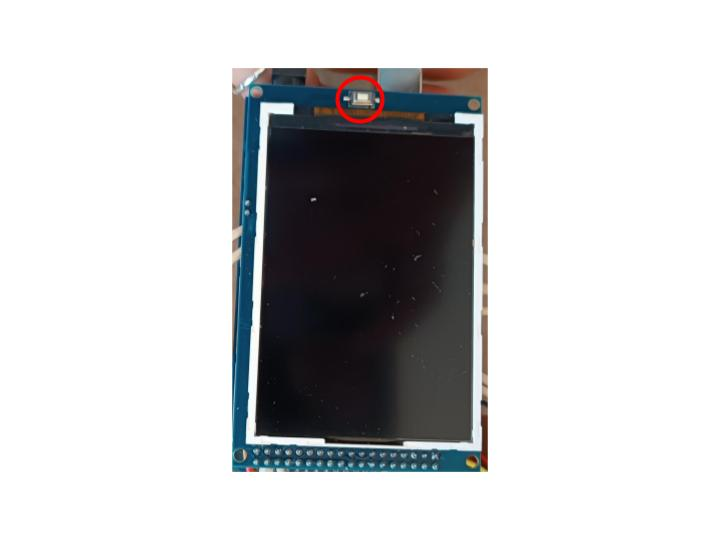
\includegraphics[width=0.5\textwidth]{../images/screen_button.jpg}
                \caption{The reset button.}
            \end{figure}
            \item Disconnect and reconnect the device to the wall.
            \item Use another cable or another adapter connected to the wall.
        \end{itemize}
        \item The buttons stop responding:
        \begin{itemize}
            \item If all buttons stop responding, try restarting the screen, as seen in the previous bullet point.
            \item If it's only one, check that the cables are in place; it is likely that a cable has become disconnected.
        \end{itemize}
\end{itemize}
\subsection{After modifying the SD cards}
\begin{itemize}
    \item The screen doesn't show any images:
    \begin{itemize}
        \item Double-check if the SD cards are in the right place (SD with images in the SD reader, SD with audio in the black MP3 player -- i.e., SD with images in the right, and SD with audio in the left).
        \item Check if the SD cards are correctly inserted. Sometimes there is still space to push it inside of the readers, i.e., check if they're ``loose''.
    \end{itemize}
\end{itemize}

\end{document}